\section{Contexte}
%\Glspl{sadapt} optimize their \glspl{behaviour} or configurations at runtime in response to a modification of their \glspl{env} or their \glspl{behaviour}~\cite{DBLP:conf/dagstuhl/ChengLGIMABBBCSDFGGGKKKLMMMPSTTWW09}.
%Kephart and Chess~\cite{DBLP:journals/computer/KephartC03} laid the groundwork for this approach, based on an IBM white paper~\cite{computing2006architectural}.
%Since then, practitioners have applied it to different domains~\cite{DBLP:journals/corr/abs-1904-01518} such as cloud infrastructure~\cite{DBLP:conf/icac/JavadiG17, OpenStack:Watcher:Wiki, DBLP:conf/icse/BarnaKFL17} or \gls{cps}~\cite{DBLP:conf/icac/LalandaGC17, DBLP:conf/cbse/FouquetMFBPJ12, DBLP:conf/smartgridsec/0001FKNT14}.
%One example of such a system is a \gls{sg}, which employs the adaptation capacity to heal itself autonomously.
%
Les systèmes auto-adaptatifs (SAS) optimisent leurs comportements ou configurations au cours de l'exécution en réponse à une modification de leur environnement ou de leurs comportements~\cite{DBLP:conf/dagstuhl/ChengLGIMABBBCSDFGGGKKKLMMMPSTTWW09}. 
Kephart et Chess~\cite{DBLP:journals/computer/KephartC03} ont défini les bases de cette approche, basée sur un livre blanc d'IBM~\cite{computing2006architectural}. 
Depuis, les praticiens l'ont appliqué à différents domaines~\cite{DBLP:journals/corr/abs-1904-01518} tels que l'infrastructure \textit{cloud}~\cite{DBLP:conf/icac/JavadiG17, OpenStack:Watcher:Wiki, DBLP:conf/icse/BarnaKFL17} ou les Système Cyber-Physique (CPS)~\cite{DBLP:conf/icac/LalandaGC17, DBLP:conf/cbse/FouquetMFBPJ12, DBLP:conf/smartgridsec/0001FKNT14}. 
Un exemple d'un tel système est un réseau intelligent, qui utilise la capacité d'adaptation pour s'auto-guérir de manière autonome.

%A \gls{sg} is a power grid in which utilities introduce \gls{ict} to face the new challenges of electricity supply~\cite{farhangi2010path, ipakchi2009grid, DBLP:journals/comsur/FangMXY12}.
%One of the required feature is the \gls{shealing} capacity.
%A \gls{shealingSyst} can automatically repair any incident, software or hardware, at runtime~\cite{DBLP:journals/computer/KephartC03}.
%For example, a smart grid can optimise the power flow to deal with failures of transformers\footnote{Transformers change the voltage in the cables.}~\cite{DBLP:journals/comsur/FangMXY12}.
%
Un réseau intelligent est un réseau électrique dans lequel les services publics ont introduit les Technologies de l'Information et de la Communication (TIC) pour faire face aux nouveaux défis de l'approvisionnement en électricité~\cite{farhangi2010path, ipakchi2009grid, DBLP:journals/comsur/FangMXY12}. 
L'une des caractéristiques requises est la capacité d'auto-guérison. 
Un système d'auto-guérison peut réparer automatiquement tout incident, logiciel ou matériel, au moment de l'exécution~\cite{DBLP:journals/computer/KephartC03}.
Par exemple, un réseau intelligent peut optimiser le flux d'énergie pour faire face aux pannes des transformateurs~\footnote{Les transformateurs modifient la tension dans les câbles.}~\cite{DBLP:journals/comsur/FangMXY12}.

%The adaptation process can be performed only if the system has a deep understanding of the situation and the problem.
%In this case, the situation comprises the \gls{structure} (elements that compose the system), the \gls{behaviour} (the set of possible \glspl{exec} of the system) and the \gls{env} (where it is executed) of the system.
%This understanding can be extracted from an, or a set of, \textbf{abstraction}(s) of these elements.
%Abstractions provide a description of systems, their \glspl{behaviour}, or their \glspl{env}.
%For example, Hartmann~\etal \cite{DBLP:conf/smartgridcomm/0001FKTPTR14} provide a class diagram that describes the smart grid topology, when it uses power lines communications\footnote{Data are sent through cables that also distribute electricity.}.
%
Le processus d'adaptation ne peut être réalisé que si le système a une connaissance approfondie de la situation et du problème. 
Dans ce cas, la situation comprend la structure (les éléments qui composent le système), le comportement (l'ensemble des exécutions possibles du système) et l'environnement (où il est exécuté) du système.
Cette compréhension peut être extraite d'une ou d'un ensemble d'abstraction(s) de ces éléments.
Les abstractions fournissent une description des systèmes, de leurs comportements ou de leur environnement. 
Par exemple, Hartmann Hartmann~\etal \cite{DBLP:conf/smartgridcomm/0001FKTPTR14} fournissent un diagramme de classes qui décrit la topologie du réseau intelligent, lorsqu'il utilise les communications par lignes électriques\footnote{Les données sont transmises par des câbles qui distribuent également l'électricité.}.

%\textbf{\Gls{mde}} defenders argue for using the abstraction mechanism to facilitate the development of current software~\cite{DBLP:journals/computer/Schmidt06, DBLP:conf/ifm/Kent02, DBLP:series/synthesis/2017Brambilla}.
%This methodology can be applied to different stages of software development.
%In this thesis, we focus on one of its paradigms: \textbf{\gls{m@rt}}~\cite{DBLP:journals/computer/BlairBF09, DBLP:journals/computer/MorinBJFS09}.
%As we depict in \Cref{fig:french:context:m@rt}, using this paradigm, the adaptation process relies on a \gls{model} for analysing the situation and triggering the adaptation.
%In this document, we say that the model represents the knowledge of the adaptation process.
%Developers can use this paradigm to implement \glspl{adptSyst}~\cite{DBLP:journals/computer/MorinBJFS09, DBLP:conf/smartgridsec/0001FKNT14}.
%This dissertation contributes to this modelling layer.
Les défenseurs de l'Ingénierie Dirigée par les Modèles (IDM) plaident pour l'utilisation du mécanisme d'abstraction pour faciliter le développement des logiciels actuels~\cite{DBLP:journals/computer/Schmidt06, DBLP:conf/ifm/Kent02, DBLP:series/synthesis/2017Brambilla}. 
Cette méthodologie peut être appliquée à différentes étapes du développement logiciel. 
Dans cette thèse, nous nous concentrons sur l'un de ses paradigmes : \textit{models@run.time}~\cite{DBLP:journals/computer/BlairBF09, DBLP:journals/computer/MorinBJFS09}. 
Comme nous l'illustrons par la~\cref{fig_french_context_m@rt}, en utilisant ce paradigme, le processus d'adaptation s'appuie sur un modèle pour analyser la situation et déclencher l'adaptation. 
Dans ce document, nous supposons que le modèle représente la connaissance du processus d'adaptation. 
Les développeurs peuvent utiliser ce paradigme pour mettre en œuvre des systèmes adaptatifs~\cite{DBLP:journals/computer/MorinBJFS09, DBLP:conf/smartgridsec/0001FKNT14}.
Cette thèse contribue à cette couche de modélisation.


\begin{figure}
	\centering
	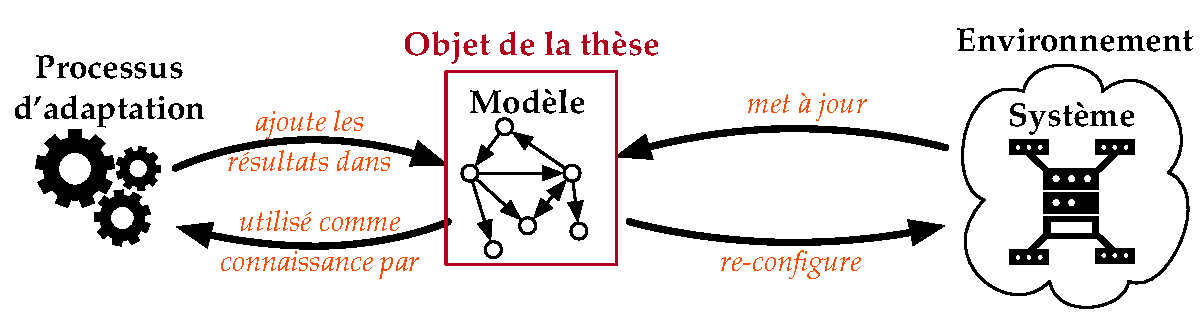
\includegraphics[width=.9\linewidth]{img/apdx-french/context/mart-focus}
	\caption{Aperçu du \gls{m@rt} et objet de la thèse}
	\label{fig_french_context_m@rt}
\end{figure}
